\documentclass[twoside]{book}

% Packages required by doxygen
\usepackage{fixltx2e}
\usepackage{calc}
\usepackage{doxygen}
\usepackage[export]{adjustbox} % also loads graphicx
\usepackage{graphicx}
\usepackage[utf8]{inputenc}
\usepackage{makeidx}
\usepackage{multicol}
\usepackage{multirow}
\PassOptionsToPackage{warn}{textcomp}
\usepackage{textcomp}
\usepackage[nointegrals]{wasysym}
\usepackage[table]{xcolor}

% Font selection
\usepackage[T1]{fontenc}
\usepackage[scaled=.90]{helvet}
\usepackage{courier}
\usepackage{amssymb}
\usepackage{sectsty}
\renewcommand{\familydefault}{\sfdefault}
\allsectionsfont{%
  \fontseries{bc}\selectfont%
  \color{darkgray}%
}
\renewcommand{\DoxyLabelFont}{%
  \fontseries{bc}\selectfont%
  \color{darkgray}%
}
\newcommand{\+}{\discretionary{\mbox{\scriptsize$\hookleftarrow$}}{}{}}

% Page & text layout
\usepackage{geometry}
\geometry{%
  a4paper,%
  top=2.5cm,%
  bottom=2.5cm,%
  left=2.5cm,%
  right=2.5cm%
}
\tolerance=750
\hfuzz=15pt
\hbadness=750
\setlength{\emergencystretch}{15pt}
\setlength{\parindent}{0cm}
\setlength{\parskip}{3ex plus 2ex minus 2ex}
\makeatletter
\renewcommand{\paragraph}{%
  \@startsection{paragraph}{4}{0ex}{-1.0ex}{1.0ex}{%
    \normalfont\normalsize\bfseries\SS@parafont%
  }%
}
\renewcommand{\subparagraph}{%
  \@startsection{subparagraph}{5}{0ex}{-1.0ex}{1.0ex}{%
    \normalfont\normalsize\bfseries\SS@subparafont%
  }%
}
\makeatother

% Headers & footers
\usepackage{fancyhdr}
\pagestyle{fancyplain}
\fancyhead[LE]{\fancyplain{}{\bfseries\thepage}}
\fancyhead[CE]{\fancyplain{}{}}
\fancyhead[RE]{\fancyplain{}{\bfseries\leftmark}}
\fancyhead[LO]{\fancyplain{}{\bfseries\rightmark}}
\fancyhead[CO]{\fancyplain{}{}}
\fancyhead[RO]{\fancyplain{}{\bfseries\thepage}}
\fancyfoot[LE]{\fancyplain{}{}}
\fancyfoot[CE]{\fancyplain{}{}}
\fancyfoot[RE]{\fancyplain{}{\bfseries\scriptsize Generated by Doxygen }}
\fancyfoot[LO]{\fancyplain{}{\bfseries\scriptsize Generated by Doxygen }}
\fancyfoot[CO]{\fancyplain{}{}}
\fancyfoot[RO]{\fancyplain{}{}}
\renewcommand{\footrulewidth}{0.4pt}
\renewcommand{\chaptermark}[1]{%
  \markboth{#1}{}%
}
\renewcommand{\sectionmark}[1]{%
  \markright{\thesection\ #1}%
}

% Indices & bibliography
\usepackage{natbib}
\usepackage[titles]{tocloft}
\setcounter{tocdepth}{3}
\setcounter{secnumdepth}{5}
\makeindex

% Hyperlinks (required, but should be loaded last)
\usepackage{ifpdf}
\ifpdf
  \usepackage[pdftex,pagebackref=true]{hyperref}
\else
  \usepackage[ps2pdf,pagebackref=true]{hyperref}
\fi
\hypersetup{%
  colorlinks=true,%
  linkcolor=blue,%
  citecolor=blue,%
  unicode%
}

% Custom commands
\newcommand{\clearemptydoublepage}{%
  \newpage{\pagestyle{empty}\cleardoublepage}%
}

\usepackage{caption}
\captionsetup{labelsep=space,justification=centering,font={bf},singlelinecheck=off,skip=4pt,position=top}

%===== C O N T E N T S =====

\begin{document}

% Titlepage & ToC
\hypersetup{pageanchor=false,
             bookmarksnumbered=true,
             pdfencoding=unicode
            }
\pagenumbering{alph}
\begin{titlepage}
\vspace*{7cm}
\begin{center}%
{\Large Sd\+Card\+Log\+Handler\+RK }\\
\vspace*{1cm}
{\large Generated by Doxygen 1.8.14}\\
\end{center}
\end{titlepage}
\clearemptydoublepage
\pagenumbering{roman}
\tableofcontents
\clearemptydoublepage
\pagenumbering{arabic}
\hypersetup{pageanchor=true}

%--- Begin generated contents ---
\chapter{Sd\+Card\+Log\+Handler\+RK}
\label{index}\hypertarget{index}{}{\itshape Library for writing rotating logs to SD card on the Particle Photon and Electron}

The \href{http://rickkas7.github.io/SdCardLogHandlerRK/}{\tt full browsable A\+PI documentation is here}.

The official location for this library is\+: \href{https://github.com/rickkas7/SdCardLogHandlerRK}{\tt https\+://github.\+com/rickkas7/\+Sd\+Card\+Log\+Handler\+RK}.

It\textquotesingle{}s in the Particle community libraries as\+: Sd\+Card\+Log\+Handler\+RK.

It\textquotesingle{}s also possible (as of version 0.\+0.\+5) to use this to write an arbitrary stream of data, not hooked into the logging A\+PI. See \mbox{\hyperlink{class_sd_card_print_handler}{Sd\+Card\+Print\+Handler}}, below.

\subsection*{Hardware}

You\textquotesingle{}ll need a SD card reader, presumably a Micro SD card reader. Make sure you get one that\textquotesingle{}s compatible with the 3.\+3V logic levels used on the Photon and Electron. Some readers designed for the Arduino expect the 5V logic levels used by the original Arduino. I use \href{https://www.sparkfun.com/products/13743}{\tt this one from Sparkfun} but there are others. \href{https://www.adafruit.com/product/254}{\tt This one from Adafruit} works as well.

  The SD card reader connects via the S\+PI interface. There are two S\+PI interfaces on the Photon and Electron and you can use either. Note that each S\+PI device must have a separate SS (sometimes called CS) pin. While it\textquotesingle{}s listed in the table below as A2 (or D5), you can use any G\+P\+IO pin.

Primary S\+PI (S\+PI object)


\begin{DoxyItemize}
\item A2 SS
\item A3 S\+CK
\item A4 M\+I\+SO
\item A5 M\+O\+SI
\end{DoxyItemize}

Secondary S\+PI (S\+P\+I1 object)


\begin{DoxyItemize}
\item D5 SS
\item D4 S\+CK
\item D3 M\+I\+SO
\item D2 M\+O\+SI
\end{DoxyItemize}

In the picture above\+:

\tabulinesep=1mm
\begin{longtabu} spread 0pt [c]{*{4}{|X[-1]}|}
\hline
\rowcolor{\tableheadbgcolor}\textbf{ Device  }&\textbf{ S\+PI Name  }&\textbf{ SD Reader  }&\textbf{ Color   }\\\cline{1-4}
\endfirsthead
\hline
\endfoot
\hline
\rowcolor{\tableheadbgcolor}\textbf{ Device  }&\textbf{ S\+PI Name  }&\textbf{ SD Reader  }&\textbf{ Color   }\\\cline{1-4}
\endhead
A2  &SS  &/\+CS  &Yellow   \\\cline{1-4}
A3  &S\+CK  &S\+CK  &Orange   \\\cline{1-4}
A4  &M\+I\+SO  &DO  &Blue   \\\cline{1-4}
A5  &M\+O\+SI  &DI  &Green   \\\cline{1-4}
3\+V3  &&V\+CC  &Red   \\\cline{1-4}
G\+ND  &&G\+ND  &Black   \\\cline{1-4}
&&CD  &\\\cline{1-4}
\end{longtabu}


\subsubsection*{Adafruit Ada\+Logger Feather\+Wing}

You can also use the \href{https://www.adafruit.com/product/2922}{\tt Adafruit Ada\+Logger Feather\+Wing}. It contains an SD card reader and a R\+TC (real-\/time clock).

 It connects to primary S\+PI (S\+PI object). The default connection is D5 for the SD card CS pin. It\textquotesingle{}s possible to cut a trace and add a jumper wire to change the CS pin.


\begin{DoxyItemize}
\item D5 CS
\item A3 S\+CK
\item A4 M\+I\+SO
\item A5 M\+O\+SI
\end{DoxyItemize}

\subsection*{Using the library}

This library uses the \href{https://docs.particle.io/reference/firmware/#logging}{\tt Logging A\+PI} that was added in system firmware 0.\+6.\+0.

For example\+:


\begin{DoxyCode}
Log.trace("Low level debugging message");
Log.info("This is info message");
Log.warn("This is warning message");
Log.error("This is error message");

Log.info("System version: %s", System.version().c\_str());
\end{DoxyCode}


It does not remap Serial, so if you\textquotesingle{}re using Serial.\+print for logging, you should switch to using Log.\+info instead.

The library creates a directory (default\+: \char`\"{}logs\char`\"{}) at the top level of the SD card and stores the log files in that. Each log file is a .txt file 6-\/digit number beginning with 000001.\+txt.

The default log file is 1 MB (1000000 bytes), but you can reconfigure this. The actual size will be slightly larger than that, as the log is rotated when it exceeds the limit, and the file will always contain a whole log entry.

When rotated, the default is to keep 10 log files, but this is configurable. The oldest is deleted when the maximum number is reached.

By default, \mbox{\hyperlink{class_sd_card_log_handler}{Sd\+Card\+Log\+Handler}} writes to Serial as well, like Serial\+Log\+Handler. This can be reconfigured.

This is the example program\+:


\begin{DoxyCode}
#include "Particle.h"

#include "SdFat.h"
#include "SdCardLogHandlerRK.h"

SYSTEM\_THREAD(ENABLED);

const int SD\_CHIP\_SELECT = A2;
SdFat sd;

SdCardLogHandler logHandler(sd, SD\_CHIP\_SELECT, SPI\_FULL\_SPEED);

size\_t counter = 0;

void setup() \{
    Serial.begin(9600);
\}

void loop() \{
    Log.info("testing counter=%d", counter++);
    delay(1000);
\}
\end{DoxyCode}


\subsubsection*{Initialize the Sd\+Fat library}

You normally initialize the Sd\+Fat library by creating a global object for it. For example\+:


\begin{DoxyCode}
SdFat sd;
\end{DoxyCode}


If you are using S\+P\+I1 (the D pins) instead, use\+:


\begin{DoxyCode}
SdFat sd(1);
\end{DoxyCode}


Note that you should not call {\ttfamily sd.\+begin()} in setup! The begin call is done by the \mbox{\hyperlink{class_sd_card_log_handler}{Sd\+Card\+Log\+Handler}} because it needs to be done earlier than setup, and also every time the card is ejected.

If you need to check for a successful call to begin in your code, instead using {\ttfamily log\+Handler.\+get\+Last\+Begin\+Result()}. You might do this before using the SD card in your code. If there is no SD card inserted, the result will be false.

\subsubsection*{Initialize the \mbox{\hyperlink{class_sd_card_log_handler}{Sd\+Card\+Log\+Handler}}}

Normally you initialize the \mbox{\hyperlink{class_sd_card_log_handler}{Sd\+Card\+Log\+Handler}} by creating a global object like this\+:


\begin{DoxyCode}
SdCardLogHandler logHandler(sd, SD\_CHIP\_SELECT, SPI\_FULL\_SPEED);
\end{DoxyCode}



\begin{DoxyItemize}
\item {\ttfamily sd} is the {\ttfamily Sd\+Fat} object, as described in the previous section
\item {\ttfamily S\+D\+\_\+\+C\+H\+I\+P\+\_\+\+S\+E\+L\+E\+CT} is the pin connected to the C\+S/\+SS pin. In the code above, {\ttfamily S\+D\+\_\+\+C\+H\+I\+P\+\_\+\+S\+E\+L\+E\+CT} is set to A2.
\item {\ttfamily S\+P\+I\+\_\+\+F\+U\+L\+L\+\_\+\+S\+P\+E\+ED} determines the speed to use, either full or {\ttfamily S\+P\+I\+\_\+\+H\+A\+L\+F\+\_\+\+S\+P\+E\+ED}.
\end{DoxyItemize}

There are also two optional parameters\+:


\begin{DoxyCode}
SdCardLogHandler logHandler(sd, SD\_CHIP\_SELECT, SPI\_FULL\_SPEED, LOG\_LEVEL\_TRACE);
\end{DoxyCode}


The next optional parameter allows you to set the logging level.


\begin{DoxyItemize}
\item {\ttfamily L\+O\+G\+\_\+\+L\+E\+V\+E\+L\+\_\+\+A\+LL} \+: special value that can be used to enable logging of all messages
\item {\ttfamily L\+O\+G\+\_\+\+L\+E\+V\+E\+L\+\_\+\+T\+R\+A\+CE} \+: verbose output for debugging purposes
\item {\ttfamily L\+O\+G\+\_\+\+L\+E\+V\+E\+L\+\_\+\+I\+N\+FO} \+: regular information messages
\item {\ttfamily L\+O\+G\+\_\+\+L\+E\+V\+E\+L\+\_\+\+W\+A\+RN} \+: warnings and non-\/critical errors
\item {\ttfamily L\+O\+G\+\_\+\+L\+E\+V\+E\+L\+\_\+\+E\+R\+R\+OR} \+: error messages
\item {\ttfamily L\+O\+G\+\_\+\+L\+E\+V\+E\+L\+\_\+\+N\+O\+NE} \+: special value that can be used to disable logging of any messages
\end{DoxyItemize}

And finally, you can use logging categories as well to set the level for certain categories\+:


\begin{DoxyCode}
SdCardLogHandler logHandler(sd, SD\_CHIP\_SELECT, SPI\_FULL\_SPEED, LOG\_LEVEL\_INFO, \{
    \{ "app.network", LOG\_LEVEL\_TRACE \} 
\});
\end{DoxyCode}


That example defaults to I\+N\+FO but app.\+network events would be at T\+R\+A\+CE level.

\subsubsection*{Using \mbox{\hyperlink{class_sd_card_print_handler}{Sd\+Card\+Print\+Handler}}}

Instead of using \mbox{\hyperlink{class_sd_card_log_handler}{Sd\+Card\+Log\+Handler}}, you can use \mbox{\hyperlink{class_sd_card_print_handler}{Sd\+Card\+Print\+Handler}}. This works like \mbox{\hyperlink{class_sd_card_log_handler}{Sd\+Card\+Log\+Handler}}, except it does not hook into the system log handler. This makes it useful for logging arbitrary data, and not have system logs mixed in.


\begin{DoxyCode}
SdCardPrintHandler printToCard(sd, SD\_CHIP\_SELECT, SPI\_FULL\_SPEED);
\end{DoxyCode}


You can use any of the print, println, or printf methods to print to the log file. The same circular log file structure is used, and the card is only written to after a ~\newline
 or println. A line is never broken up across multiple files.


\begin{DoxyCode}
printToCard.println("testing!");
\end{DoxyCode}


\subsubsection*{Options}

The options below work with both \mbox{\hyperlink{class_sd_card_log_handler}{Sd\+Card\+Log\+Handler}} and \mbox{\hyperlink{class_sd_card_print_handler}{Sd\+Card\+Print\+Handler}}.

There are also options available to control how logging is done. For example, if you want to change the default log file size to (approximately) 50000 bytes\+:


\begin{DoxyCode}
SdCardLogHandler logHandler(sd, SD\_CHIP\_SELECT, SPI\_FULL\_SPEED, LOG\_LEVEL\_TRACE);
STARTUP(logHandler.withDesiredFileSize(50000));
\end{DoxyCode}


You can chain these together fluent-\/style to change multiple settings\+:


\begin{DoxyCode}
SdCardLogHandler logHandler(sd, SD\_CHIP\_SELECT, SPI\_FULL\_SPEED, LOG\_LEVEL\_TRACE);
STARTUP(logHandler.withDesiredFileSize(50000).withMaxFilesToKeep(5));
\end{DoxyCode}


By default, \mbox{\hyperlink{class_sd_card_log_handler}{Sd\+Card\+Log\+Handler}} writes the log entries to Serial like Serial\+Log\+Handler. You can turn this off by using\+:


\begin{DoxyCode}
SdCardLogHandler logHandler(sd, SD\_CHIP\_SELECT, SPI\_FULL\_SPEED, LOG\_LEVEL\_TRACE);
STARTUP(logHandler.withNoSerialLogging());
\end{DoxyCode}


Or if you want to log to Serial1 (or another port) instead\+:


\begin{DoxyCode}
SdCardLogHandler logHandler(sd, SD\_CHIP\_SELECT, SPI\_FULL\_SPEED, LOG\_LEVEL\_TRACE);
STARTUP(logHandler.withWriteToStream(&Serial1);
\end{DoxyCode}


Normally, a sync operation is done after each log entry, which maximizes the chance the the log entry will be written out to SD card successfully. However, this will slow down operation if you do a lot of logging. You can have the Sd\+Fat library manage its own sync, which happens about every 512 bytes of log messages, by turning off sync after every entry\+:


\begin{DoxyCode}
SdCardLogHandler logHandler(sd, SD\_CHIP\_SELECT, SPI\_FULL\_SPEED, LOG\_LEVEL\_TRACE);
STARTUP(logHandler.withSyncEveryEntry(false);
\end{DoxyCode}


Finally, when the SD card is ejected, a check for being inserted is only done at most every 10 seconds. This is because there\textquotesingle{}s a timeout operation that makes the operation slow, and doing it on every log entry would make the performance very bad. You can change this interval by using\+:


\begin{DoxyCode}
SdCardLogHandler logHandler(sd, SD\_CHIP\_SELECT, SPI\_FULL\_SPEED, LOG\_LEVEL\_TRACE);
STARTUP(logHandler.withCardCheckPeriod(30000);
\end{DoxyCode}


The value is in milliseconds; that changes the value from 10 seconds to 30 seconds. 
\chapter{Hierarchical Index}
\section{Class Hierarchy}
This inheritance list is sorted roughly, but not completely, alphabetically\+:\begin{DoxyCompactList}
\item Print\begin{DoxyCompactList}
\item \contentsline{section}{Sd\+Card\+Print\+Handler}{\pageref{class_sd_card_print_handler}}{}
\begin{DoxyCompactList}
\item \contentsline{section}{Sd\+Card\+Log\+Handler}{\pageref{class_sd_card_log_handler}}{}
\end{DoxyCompactList}
\end{DoxyCompactList}
\item Stream\+Log\+Handler\begin{DoxyCompactList}
\item \contentsline{section}{Sd\+Card\+Log\+Handler}{\pageref{class_sd_card_log_handler}}{}
\end{DoxyCompactList}
\end{DoxyCompactList}

\chapter{Data Structure Index}
\section{Data Structures}
Here are the data structures with brief descriptions\+:\begin{DoxyCompactList}
\item\contentsline{section}{\mbox{\hyperlink{class_sd_card_log_handler}{Sd\+Card\+Log\+Handler}} \\*Class for logging to SD card }{\pageref{class_sd_card_log_handler}}{}
\item\contentsline{section}{\mbox{\hyperlink{class_sd_card_print_handler}{Sd\+Card\+Print\+Handler}} \\*Class for writing a data stream to SD card }{\pageref{class_sd_card_print_handler}}{}
\end{DoxyCompactList}

\chapter{Data Structure Documentation}
\hypertarget{class_sd_card_log_handler}{}\section{Sd\+Card\+Log\+Handler Class Reference}
\label{class_sd_card_log_handler}\index{Sd\+Card\+Log\+Handler@{Sd\+Card\+Log\+Handler}}


Class for logging to SD card.  




{\ttfamily \#include $<$Sd\+Card\+Log\+Handler\+R\+K.\+h$>$}

Inheritance diagram for Sd\+Card\+Log\+Handler\+:\begin{figure}[H]
\begin{center}
\leavevmode
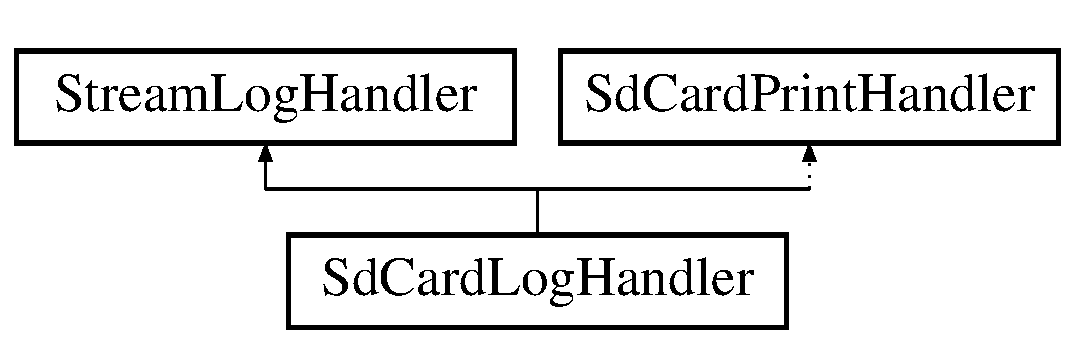
\includegraphics[height=2.000000cm]{class_sd_card_log_handler}
\end{center}
\end{figure}
\subsection*{Public Member Functions}
\begin{DoxyCompactItemize}
\item 
\mbox{\hyperlink{class_sd_card_log_handler_a307fc19ae158016fa223b245210a050c}{Sd\+Card\+Log\+Handler}} (Sd\+Fat \&sd, uint8\+\_\+t cs\+Pin, uint8\+\_\+t divisor, Log\+Level level=L\+O\+G\+\_\+\+L\+E\+V\+E\+L\+\_\+\+I\+N\+FO, Log\+Category\+Filters filters=\{\})
\begin{DoxyCompactList}\small\item\em Constructor. The object is normally instantiated as a global object. \end{DoxyCompactList}\item 
\mbox{\Hypertarget{class_sd_card_log_handler_aaf48dcdc1f7b0965e66cbc976f4e12e0}\label{class_sd_card_log_handler_aaf48dcdc1f7b0965e66cbc976f4e12e0}} 
virtual size\+\_\+t \mbox{\hyperlink{class_sd_card_log_handler_aaf48dcdc1f7b0965e66cbc976f4e12e0}{write}} (uint8\+\_\+t)
\begin{DoxyCompactList}\small\item\em Virtual override for the Stream\+Log\+Handler to write data to the log. \end{DoxyCompactList}\end{DoxyCompactItemize}


\subsection{Detailed Description}
Class for logging to SD card. 

You normally instantiate one of these as a global variable, passing in the Sd\+Fat object and the parameters you\textquotesingle{}d normally pass to Sd\+Fat\+::begin(). You can optionally pass the Log\+Level and Log\+Category\+Filters parameters you\textquotesingle{}d pass to the Log\+Handler constructor.


\begin{DoxyCode}
\textcolor{keyword}{const} \textcolor{keywordtype}{int} SD\_CHIP\_SELECT = A2;
SdFat sd;

\mbox{\hyperlink{class_sd_card_log_handler}{SdCardLogHandler}} logHandler(sd, SD\_CHIP\_SELECT, SPI\_FULL\_SPEED);
\end{DoxyCode}


You can pass additional options using the fluent-\/style methods beginning with \char`\"{}with\char`\"{} like \mbox{\hyperlink{class_sd_card_print_handler_aac9a7f9d1a22db39acfc17c4a61c9419}{with\+Logs\+Dir\+Name()}}. 

\subsection{Constructor \& Destructor Documentation}
\mbox{\Hypertarget{class_sd_card_log_handler_a307fc19ae158016fa223b245210a050c}\label{class_sd_card_log_handler_a307fc19ae158016fa223b245210a050c}} 
\index{Sd\+Card\+Log\+Handler@{Sd\+Card\+Log\+Handler}!Sd\+Card\+Log\+Handler@{Sd\+Card\+Log\+Handler}}
\index{Sd\+Card\+Log\+Handler@{Sd\+Card\+Log\+Handler}!Sd\+Card\+Log\+Handler@{Sd\+Card\+Log\+Handler}}
\subsubsection{\texorpdfstring{Sd\+Card\+Log\+Handler()}{SdCardLogHandler()}}
{\footnotesize\ttfamily Sd\+Card\+Log\+Handler\+::\+Sd\+Card\+Log\+Handler (\begin{DoxyParamCaption}\item[{Sd\+Fat \&}]{sd,  }\item[{uint8\+\_\+t}]{cs\+Pin,  }\item[{uint8\+\_\+t}]{divisor,  }\item[{Log\+Level}]{level = {\ttfamily LOG\+\_\+LEVEL\+\_\+INFO},  }\item[{Log\+Category\+Filters}]{filters = {\ttfamily \{\}} }\end{DoxyParamCaption})}



Constructor. The object is normally instantiated as a global object. 


\begin{DoxyParams}{Parameters}
{\em sd} & The Sd\+Fat object, normally allocated a global object. \\
\hline
{\em cs\+Pin} & The pin used for the S\+PI chip select for the SD card reader \\
\hline
{\em divisor} & Usually either S\+P\+I\+\_\+\+F\+U\+L\+L\+\_\+\+S\+P\+E\+ED or S\+P\+I\+\_\+\+H\+A\+L\+F\+\_\+\+S\+P\+E\+ED. \\
\hline
{\em level} & (optional, default is L\+O\+G\+\_\+\+L\+E\+V\+E\+L\+\_\+\+I\+N\+FO) \\
\hline
{\em filters} & (optional, default is none) \\
\hline
\end{DoxyParams}


The documentation for this class was generated from the following files\+:\begin{DoxyCompactItemize}
\item 
src/Sd\+Card\+Log\+Handler\+R\+K.\+h\item 
src/Sd\+Card\+Log\+Handler\+R\+K.\+cpp\end{DoxyCompactItemize}

\hypertarget{class_sd_card_print_handler}{}\section{Sd\+Card\+Print\+Handler Class Reference}
\label{class_sd_card_print_handler}\index{Sd\+Card\+Print\+Handler@{Sd\+Card\+Print\+Handler}}


Class for writing a data stream to SD card.  




{\ttfamily \#include $<$Sd\+Card\+Log\+Handler\+R\+K.\+h$>$}

Inheritance diagram for Sd\+Card\+Print\+Handler\+:\begin{figure}[H]
\begin{center}
\leavevmode
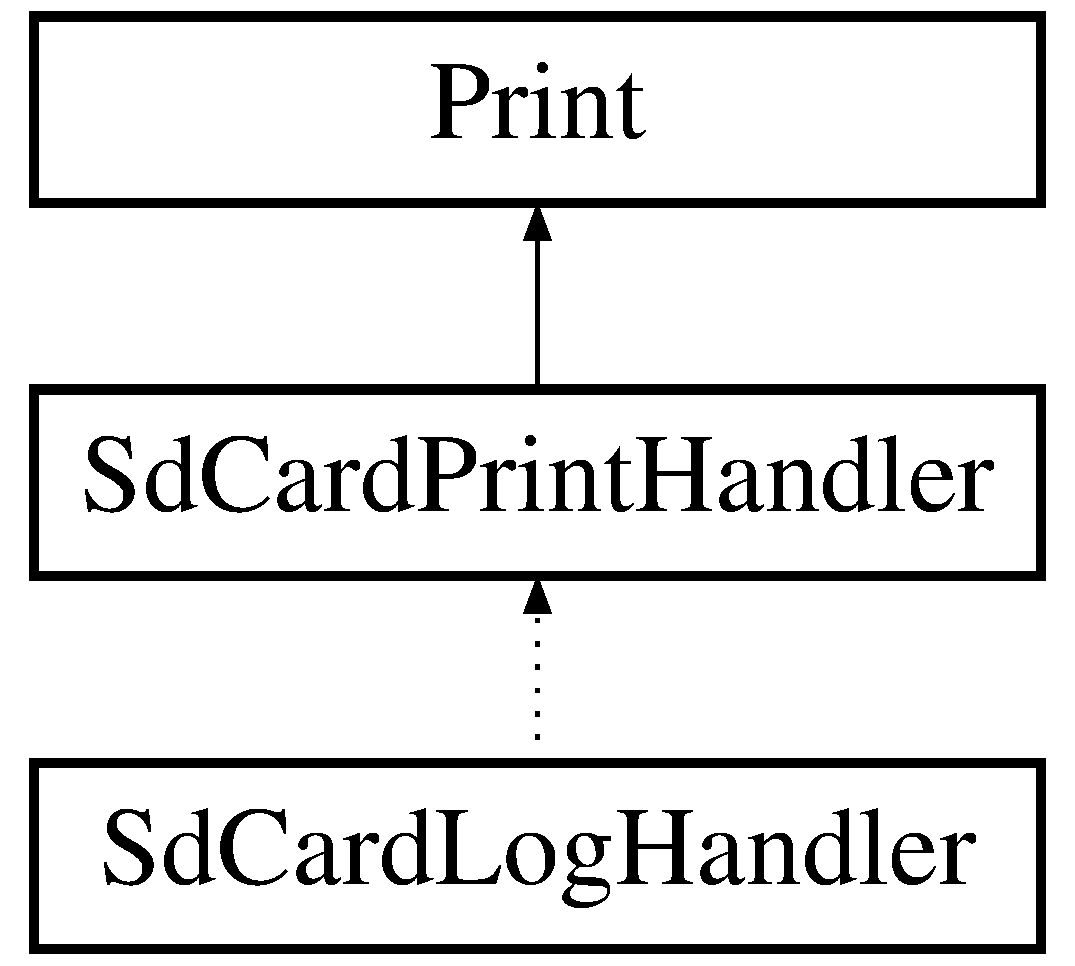
\includegraphics[height=3.000000cm]{class_sd_card_print_handler}
\end{center}
\end{figure}
\subsection*{Public Member Functions}
\begin{DoxyCompactItemize}
\item 
\mbox{\Hypertarget{class_sd_card_print_handler_a1e9332a9b5a9a5a93a89d55dc8ee8c56}\label{class_sd_card_print_handler_a1e9332a9b5a9a5a93a89d55dc8ee8c56}} 
{\bfseries Sd\+Card\+Print\+Handler} (Sd\+Fat \&sd, uint8\+\_\+t cs\+Pin, uint8\+\_\+t divisor)
\item 
\mbox{\hyperlink{class_sd_card_print_handler}{Sd\+Card\+Print\+Handler}} \& \mbox{\hyperlink{class_sd_card_print_handler_aac9a7f9d1a22db39acfc17c4a61c9419}{with\+Logs\+Dir\+Name}} (const char $\ast$value)
\begin{DoxyCompactList}\small\item\em Sets the log directory name. Default\+: \char`\"{}logs\char`\"{}. \end{DoxyCompactList}\item 
\mbox{\hyperlink{class_sd_card_print_handler}{Sd\+Card\+Print\+Handler}} \& \mbox{\hyperlink{class_sd_card_print_handler_a72ba4425d0d1551a2ad4513f2bfaefa5}{with\+Desired\+File\+Size}} (size\+\_\+t value)
\begin{DoxyCompactList}\small\item\em Desired file size in bytes. Default\+: 1000000 bytes (1 MB) \end{DoxyCompactList}\item 
\mbox{\hyperlink{class_sd_card_print_handler}{Sd\+Card\+Print\+Handler}} \& \mbox{\hyperlink{class_sd_card_print_handler_a8b0884db89c62250822641cde11a5abc}{with\+Max\+Files\+To\+Keep}} (size\+\_\+t value)
\begin{DoxyCompactList}\small\item\em The number of files to keep. Default\+: 10. \end{DoxyCompactList}\item 
\mbox{\hyperlink{class_sd_card_print_handler}{Sd\+Card\+Print\+Handler}} \& \mbox{\hyperlink{class_sd_card_print_handler_a0ddcaed71e575f70e5a5240cd5765002}{with\+Card\+Check\+Period}} (unsigned long value)
\begin{DoxyCompactList}\small\item\em The number of milliseconds to between checks to see if the SD card is present. Default\+: 10000. \end{DoxyCompactList}\item 
\mbox{\hyperlink{class_sd_card_print_handler}{Sd\+Card\+Print\+Handler}} \& \mbox{\hyperlink{class_sd_card_print_handler_a9172a9620d575738e1387005e16759f9}{with\+Sync\+Every\+Entry}} (size\+\_\+t value)
\begin{DoxyCompactList}\small\item\em Set whether to sync the file system after every log entry. Default\+: true. \end{DoxyCompactList}\item 
\mbox{\hyperlink{class_sd_card_print_handler}{Sd\+Card\+Print\+Handler}} \& \mbox{\hyperlink{class_sd_card_print_handler_a4c3cac5a8a622e51ce43d5942dc47c7a}{with\+No\+Serial\+Logging}} ()
\begin{DoxyCompactList}\small\item\em The default is to log to Serial as well as SD card; to only log to SD card call this method. \end{DoxyCompactList}\item 
\mbox{\hyperlink{class_sd_card_print_handler}{Sd\+Card\+Print\+Handler}} \& \mbox{\hyperlink{class_sd_card_print_handler_acdb2ef1ae77acdfd9c3d355548c94750}{with\+Write\+To\+Stream}} (Stream $\ast$value)
\begin{DoxyCompactList}\small\item\em Write to a different Stream, such as Serial1. Default\+: Serial. \end{DoxyCompactList}\item 
\mbox{\Hypertarget{class_sd_card_print_handler_adf54a74997d6fd7e9043199d0237c4ea}\label{class_sd_card_print_handler_adf54a74997d6fd7e9043199d0237c4ea}} 
virtual size\+\_\+t \mbox{\hyperlink{class_sd_card_print_handler_adf54a74997d6fd7e9043199d0237c4ea}{write}} (uint8\+\_\+t)
\begin{DoxyCompactList}\small\item\em Virtual override for the Stream\+Log\+Handler to write data to the log. \end{DoxyCompactList}\item 
bool \mbox{\hyperlink{class_sd_card_print_handler_ab8e7ac1b3c60f5545ea297e2f04b9ccf}{get\+Last\+Begin\+Result}} () const
\begin{DoxyCompactList}\small\item\em Checks the result of the last time sd.\+begin() was called. \end{DoxyCompactList}\end{DoxyCompactItemize}


\subsection{Detailed Description}
Class for writing a data stream to SD card. 

You normally instantiate one of these as a global variable, passing in the Sd\+Fat object and the parameters you\textquotesingle{}d normally pass to Sd\+Fat\+::begin().


\begin{DoxyCode}
\textcolor{keyword}{const} \textcolor{keywordtype}{int} SD\_CHIP\_SELECT = A2;
SdFat sd;

\mbox{\hyperlink{class_sd_card_log_handler}{SdCardLogHandler}} logHandler(sd, SD\_CHIP\_SELECT, SPI\_FULL\_SPEED);
\end{DoxyCode}


You can pass additional options using the fluent-\/style methods beginning with \char`\"{}with\char`\"{} like \mbox{\hyperlink{class_sd_card_print_handler_aac9a7f9d1a22db39acfc17c4a61c9419}{with\+Logs\+Dir\+Name()}}.

This class is a subclass of Print, so you can use all of the overloads of print, println, and printf that are supported by Print. Data is buffered until the ~\newline
, then written to the card, for performance reasons and to avoid splitting a line between multiple files. 

\subsection{Member Function Documentation}
\mbox{\Hypertarget{class_sd_card_print_handler_ab8e7ac1b3c60f5545ea297e2f04b9ccf}\label{class_sd_card_print_handler_ab8e7ac1b3c60f5545ea297e2f04b9ccf}} 
\index{Sd\+Card\+Print\+Handler@{Sd\+Card\+Print\+Handler}!get\+Last\+Begin\+Result@{get\+Last\+Begin\+Result}}
\index{get\+Last\+Begin\+Result@{get\+Last\+Begin\+Result}!Sd\+Card\+Print\+Handler@{Sd\+Card\+Print\+Handler}}
\subsubsection{\texorpdfstring{get\+Last\+Begin\+Result()}{getLastBeginResult()}}
{\footnotesize\ttfamily bool Sd\+Card\+Print\+Handler\+::get\+Last\+Begin\+Result (\begin{DoxyParamCaption}{ }\end{DoxyParamCaption}) const\hspace{0.3cm}{\ttfamily [inline]}}



Checks the result of the last time sd.\+begin() was called. 

This call determines whether the last call to sd.\+begin() succeeded or not. You might do this if you also need to call Sd\+Fat from your own code. This library needs to call sd.\+begin() internally to do it very early, and also after the SD card is ejected.

\begin{DoxyReturn}{Returns}
true if begin was successful 
\end{DoxyReturn}
\mbox{\Hypertarget{class_sd_card_print_handler_a0ddcaed71e575f70e5a5240cd5765002}\label{class_sd_card_print_handler_a0ddcaed71e575f70e5a5240cd5765002}} 
\index{Sd\+Card\+Print\+Handler@{Sd\+Card\+Print\+Handler}!with\+Card\+Check\+Period@{with\+Card\+Check\+Period}}
\index{with\+Card\+Check\+Period@{with\+Card\+Check\+Period}!Sd\+Card\+Print\+Handler@{Sd\+Card\+Print\+Handler}}
\subsubsection{\texorpdfstring{with\+Card\+Check\+Period()}{withCardCheckPeriod()}}
{\footnotesize\ttfamily \mbox{\hyperlink{class_sd_card_print_handler}{Sd\+Card\+Print\+Handler}}\& Sd\+Card\+Print\+Handler\+::with\+Card\+Check\+Period (\begin{DoxyParamCaption}\item[{unsigned long}]{value }\end{DoxyParamCaption})\hspace{0.3cm}{\ttfamily [inline]}}



The number of milliseconds to between checks to see if the SD card is present. Default\+: 10000. 

When you remove the SD card, it\textquotesingle{}s necessary to reinitialize the Sd\+Fat library and check for the card. Because of timeouts, this takes a while, so logging would become very slow if every attempt to log caused this delay. The card check period reduces the frequency of checking to see if a card has been inserted.

Note that as long as you leave the card in, you won\textquotesingle{}t experience this.


\begin{DoxyParams}{Parameters}
{\em value} & The time in milliseconds (unsigned ling) \\
\hline
\end{DoxyParams}
\mbox{\Hypertarget{class_sd_card_print_handler_a72ba4425d0d1551a2ad4513f2bfaefa5}\label{class_sd_card_print_handler_a72ba4425d0d1551a2ad4513f2bfaefa5}} 
\index{Sd\+Card\+Print\+Handler@{Sd\+Card\+Print\+Handler}!with\+Desired\+File\+Size@{with\+Desired\+File\+Size}}
\index{with\+Desired\+File\+Size@{with\+Desired\+File\+Size}!Sd\+Card\+Print\+Handler@{Sd\+Card\+Print\+Handler}}
\subsubsection{\texorpdfstring{with\+Desired\+File\+Size()}{withDesiredFileSize()}}
{\footnotesize\ttfamily \mbox{\hyperlink{class_sd_card_print_handler}{Sd\+Card\+Print\+Handler}}\& Sd\+Card\+Print\+Handler\+::with\+Desired\+File\+Size (\begin{DoxyParamCaption}\item[{size\+\_\+t}]{value }\end{DoxyParamCaption})\hspace{0.3cm}{\ttfamily [inline]}}



Desired file size in bytes. Default\+: 1000000 bytes (1 MB) 

Each log file will be approximately this size. It typically will be slightly larger than this, as the log is rotated when the size is exceeded. If changed, it will only be enforced for the current log file; old log files are not modified.


\begin{DoxyParams}{Parameters}
{\em value} & The maximum file size for a log file in bytes (size\+\_\+t) \\
\hline
\end{DoxyParams}
\mbox{\Hypertarget{class_sd_card_print_handler_aac9a7f9d1a22db39acfc17c4a61c9419}\label{class_sd_card_print_handler_aac9a7f9d1a22db39acfc17c4a61c9419}} 
\index{Sd\+Card\+Print\+Handler@{Sd\+Card\+Print\+Handler}!with\+Logs\+Dir\+Name@{with\+Logs\+Dir\+Name}}
\index{with\+Logs\+Dir\+Name@{with\+Logs\+Dir\+Name}!Sd\+Card\+Print\+Handler@{Sd\+Card\+Print\+Handler}}
\subsubsection{\texorpdfstring{with\+Logs\+Dir\+Name()}{withLogsDirName()}}
{\footnotesize\ttfamily \mbox{\hyperlink{class_sd_card_print_handler}{Sd\+Card\+Print\+Handler}}\& Sd\+Card\+Print\+Handler\+::with\+Logs\+Dir\+Name (\begin{DoxyParamCaption}\item[{const char $\ast$}]{value }\end{DoxyParamCaption})\hspace{0.3cm}{\ttfamily [inline]}}



Sets the log directory name. Default\+: \char`\"{}logs\char`\"{}. 

The logs must always be in a subdirectory, so make sure you set it to something, setting it to an empty string or N\+U\+LL will disable logging.


\begin{DoxyParams}{Parameters}
{\em value} & The name to use instead of \char`\"{}logs\char`\"{} (const char $\ast$). This is not copied, as a constant string is normally passed in. If you calculate it, make sure you put it in a static or allocated buffer! \\
\hline
\end{DoxyParams}
\mbox{\Hypertarget{class_sd_card_print_handler_a8b0884db89c62250822641cde11a5abc}\label{class_sd_card_print_handler_a8b0884db89c62250822641cde11a5abc}} 
\index{Sd\+Card\+Print\+Handler@{Sd\+Card\+Print\+Handler}!with\+Max\+Files\+To\+Keep@{with\+Max\+Files\+To\+Keep}}
\index{with\+Max\+Files\+To\+Keep@{with\+Max\+Files\+To\+Keep}!Sd\+Card\+Print\+Handler@{Sd\+Card\+Print\+Handler}}
\subsubsection{\texorpdfstring{with\+Max\+Files\+To\+Keep()}{withMaxFilesToKeep()}}
{\footnotesize\ttfamily \mbox{\hyperlink{class_sd_card_print_handler}{Sd\+Card\+Print\+Handler}}\& Sd\+Card\+Print\+Handler\+::with\+Max\+Files\+To\+Keep (\begin{DoxyParamCaption}\item[{size\+\_\+t}]{value }\end{DoxyParamCaption})\hspace{0.3cm}{\ttfamily [inline]}}



The number of files to keep. Default\+: 10. 

The maximum number of log files to keep is enforced at startup, when a SD card is inserted, and when the current log file is full.


\begin{DoxyParams}{Parameters}
{\em value} & Number of files to kee. Values are 1 $<$= num $<$= 999999 (size\+\_\+t) \\
\hline
\end{DoxyParams}
\mbox{\Hypertarget{class_sd_card_print_handler_a4c3cac5a8a622e51ce43d5942dc47c7a}\label{class_sd_card_print_handler_a4c3cac5a8a622e51ce43d5942dc47c7a}} 
\index{Sd\+Card\+Print\+Handler@{Sd\+Card\+Print\+Handler}!with\+No\+Serial\+Logging@{with\+No\+Serial\+Logging}}
\index{with\+No\+Serial\+Logging@{with\+No\+Serial\+Logging}!Sd\+Card\+Print\+Handler@{Sd\+Card\+Print\+Handler}}
\subsubsection{\texorpdfstring{with\+No\+Serial\+Logging()}{withNoSerialLogging()}}
{\footnotesize\ttfamily \mbox{\hyperlink{class_sd_card_print_handler}{Sd\+Card\+Print\+Handler}}\& Sd\+Card\+Print\+Handler\+::with\+No\+Serial\+Logging (\begin{DoxyParamCaption}{ }\end{DoxyParamCaption})\hspace{0.3cm}{\ttfamily [inline]}}



The default is to log to Serial as well as SD card; to only log to SD card call this method. 

If you want to log to a different stream (like Serial1), use \mbox{\hyperlink{class_sd_card_print_handler_acdb2ef1ae77acdfd9c3d355548c94750}{with\+Write\+To\+Stream()}} instead. \mbox{\Hypertarget{class_sd_card_print_handler_a9172a9620d575738e1387005e16759f9}\label{class_sd_card_print_handler_a9172a9620d575738e1387005e16759f9}} 
\index{Sd\+Card\+Print\+Handler@{Sd\+Card\+Print\+Handler}!with\+Sync\+Every\+Entry@{with\+Sync\+Every\+Entry}}
\index{with\+Sync\+Every\+Entry@{with\+Sync\+Every\+Entry}!Sd\+Card\+Print\+Handler@{Sd\+Card\+Print\+Handler}}
\subsubsection{\texorpdfstring{with\+Sync\+Every\+Entry()}{withSyncEveryEntry()}}
{\footnotesize\ttfamily \mbox{\hyperlink{class_sd_card_print_handler}{Sd\+Card\+Print\+Handler}}\& Sd\+Card\+Print\+Handler\+::with\+Sync\+Every\+Entry (\begin{DoxyParamCaption}\item[{size\+\_\+t}]{value }\end{DoxyParamCaption})\hspace{0.3cm}{\ttfamily [inline]}}



Set whether to sync the file system after every log entry. Default\+: true. 

Setting this to false dramatically improves the performance, but it also makes it much more likely that in the case of a reboot, the last log messages will be lost. The Sd\+Fat library normally only flushes the file in 512 byte increments so if you log infrequently, you could lose a number of log messages.


\begin{DoxyParams}{Parameters}
{\em value} & The value to set (size\+\_\+t) \\
\hline
\end{DoxyParams}
\mbox{\Hypertarget{class_sd_card_print_handler_acdb2ef1ae77acdfd9c3d355548c94750}\label{class_sd_card_print_handler_acdb2ef1ae77acdfd9c3d355548c94750}} 
\index{Sd\+Card\+Print\+Handler@{Sd\+Card\+Print\+Handler}!with\+Write\+To\+Stream@{with\+Write\+To\+Stream}}
\index{with\+Write\+To\+Stream@{with\+Write\+To\+Stream}!Sd\+Card\+Print\+Handler@{Sd\+Card\+Print\+Handler}}
\subsubsection{\texorpdfstring{with\+Write\+To\+Stream()}{withWriteToStream()}}
{\footnotesize\ttfamily \mbox{\hyperlink{class_sd_card_print_handler}{Sd\+Card\+Print\+Handler}}\& Sd\+Card\+Print\+Handler\+::with\+Write\+To\+Stream (\begin{DoxyParamCaption}\item[{Stream $\ast$}]{value }\end{DoxyParamCaption})\hspace{0.3cm}{\ttfamily [inline]}}



Write to a different Stream, such as Serial1. Default\+: Serial. 


\begin{DoxyParams}{Parameters}
{\em value} & The stream to write log output to (such as \&Serial1) or N\+U\+LL to only write to the SD card.\\
\hline
\end{DoxyParams}
Only one stream is supported. Setting it again replaces the last setting. 

The documentation for this class was generated from the following files\+:\begin{DoxyCompactItemize}
\item 
src/Sd\+Card\+Log\+Handler\+R\+K.\+h\item 
src/Sd\+Card\+Log\+Handler\+R\+K.\+cpp\end{DoxyCompactItemize}

%--- End generated contents ---

% Index
\backmatter
\newpage
\phantomsection
\clearemptydoublepage
\addcontentsline{toc}{chapter}{Index}
\printindex

\end{document}
